\chapter{Approach}

\section{Quadrotor Platform}
Because the design and construction of a quadrotor is beyond the scope of  this project, we will use a commercially available vehicle called the Bitcraze Crazyflie \cite{bitcraze}. The Crazyflie, shown in Figure \ref{fig:quad} is a small, low cost, open-source quadrotor kit suitable for indoor flight. It measures 9 cm motor to motor and weighs 19 grams. A 170 mAh lithium-polymer battery powers the vehicle, providing 7 minutes of flight time. An onboard microcontroller is responsible for vehicle stabilization and control and reads sensor measurements from a three-axis accelerometer and a three-axis gyroscope.
\begin{figure}[!htb]
\centering 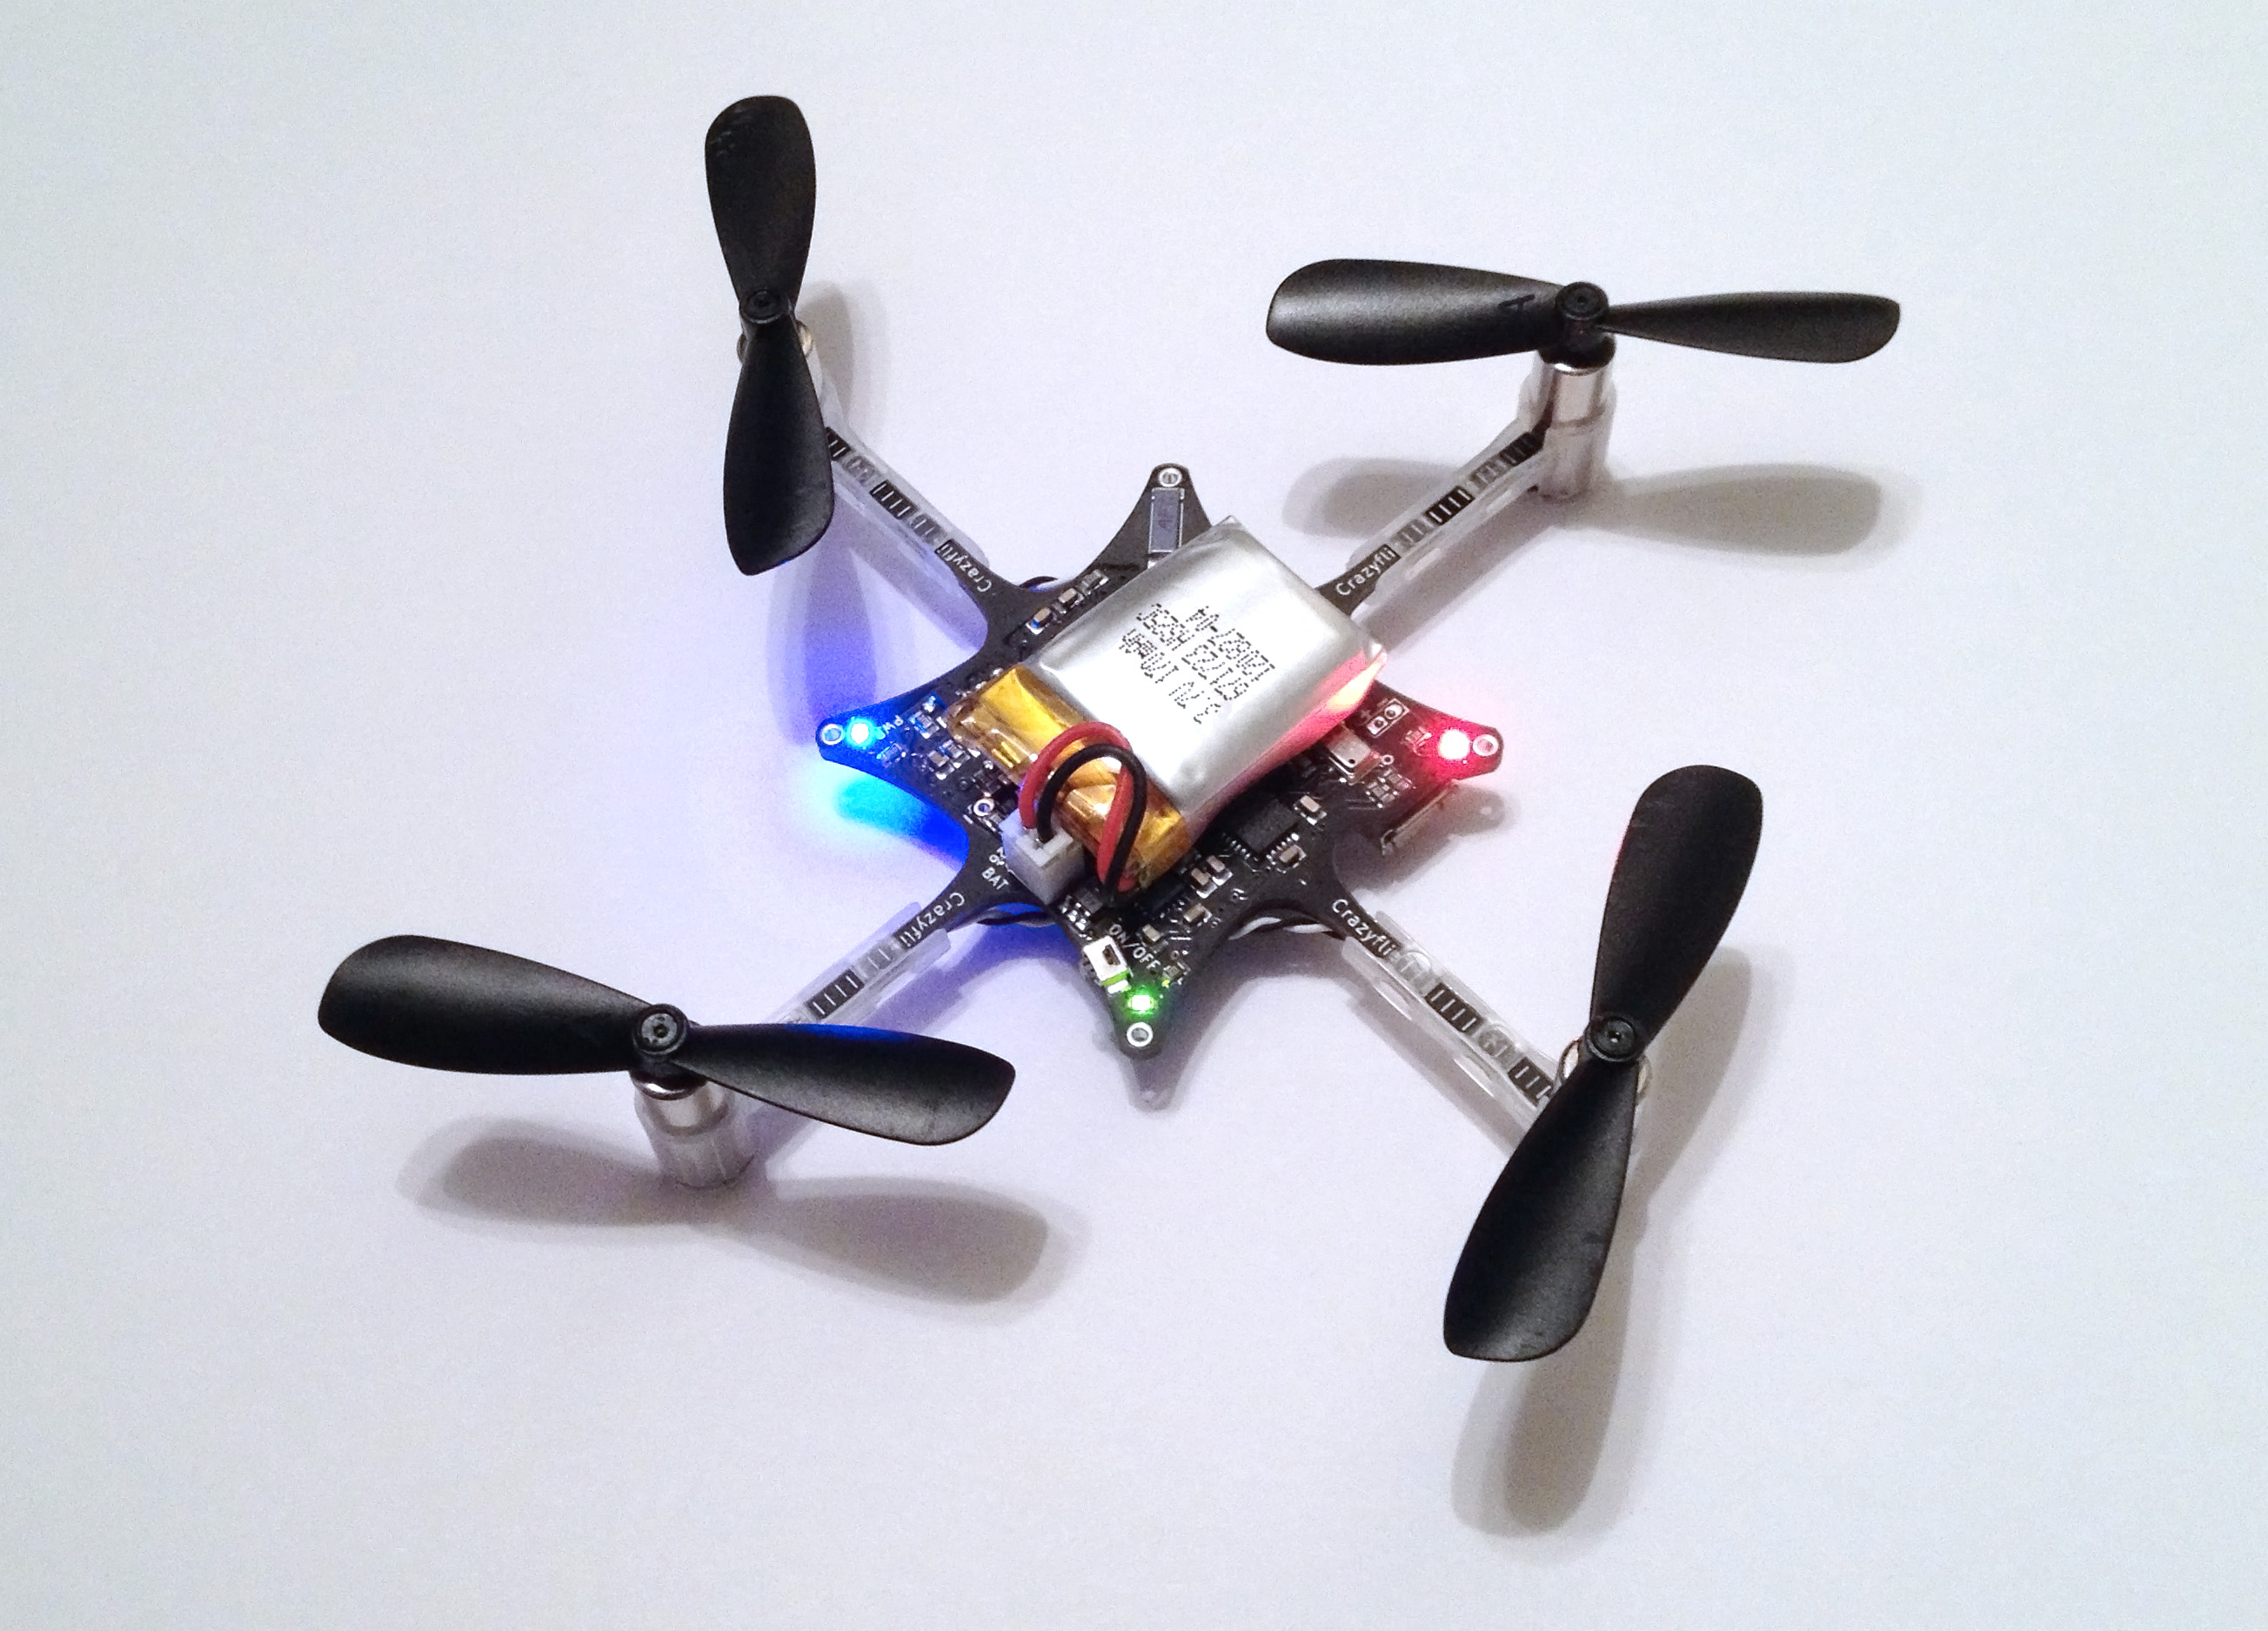
\includegraphics[scale=.11]{../fig/crazyflie.jpg}
\caption{Bitcraze Crazyflie Quadrotor}
\label{fig:quad}
\end{figure}

Vehicle pitch, roll, yaw, and thrust inputs are set in one of two ways. First, a USB gamepad connected to a computer running the Crazyflie PC client provides a method for direct user control of the vehicle. Second, the PC client exposes a Python API, making it possible to programmatically send the vehicle control set-points. The vehicle receives control inputs and transmits telemetry data wirelessly over a 2.4 GHz radio connection to a USB radio dongle connected to the Crazyflie PC client running on a laptop computer.

The onboard stabilization and control system implements an outer-loop attitude controller and an inner-loop rate controller, as shown in Figure \ref{fig:control_system_block_diagram}. Reference pitch and roll commands ($\phi$ and $\theta$, respectively) are fed to the attitude controller (outputting desired rates) and reference yaw rate ($\dot\psi$) is fed directly to the rate controller. The inner-loop rate control operates at 500 Hz and the outer-loop attitude control operates at 250 Hz.
\begin{figure}[htb!]
	\centering
	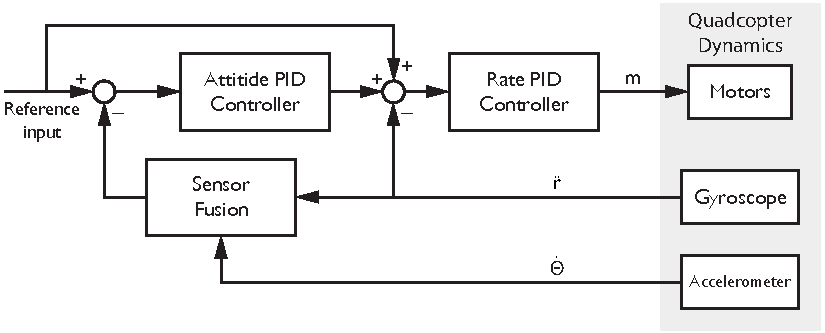
\includegraphics{../fig/crazyflie_control_system_block_diagram.pdf}
	\caption[Crazyflie stabilization and control system block diagram.]{Crazyflie stabilization and control system block diagram where $m = \begin{bmatrix}m_1 & m_2 & m_3 & m_4\end{bmatrix}^T$ is a vector of motor commands, $\ddot{r} = \begin{bmatrix}\ddot{x}&\ddot{y}&\ddot{z}\end{bmatrix}^T$ is a vector of inertial-frame accelerations, and $\dot\Theta = \begin{bmatrix}\dot{p}&\dot{q}&\dot{r}\end{bmatrix}^T$ is a vector of inertial-frame angular rotation rates.}
	\label{fig:control_system_block_diagram}
\end{figure}


\section{Experiment Design}
A crucial step in system identification is experiment design. In order to develop a robust system model, the input sequence must sufficiently excite all system modes to be identified and the sensor data must be sampled fast enough to avoid aliasing. Because the choices made during experiment design have a direct impact on the identified model, it may be necessary to update aspects of the design if the model is found to be insufficient. In this sense, the development of a system model through system identification may be viewed as an iterative procedure.

\subsection{Input Design}
The input sequence plays an important role in system identification by providing a mechanism by which the unknown system is excited, allowing us to capture system input-output data required by the identification problem. Common input sequences used for system identification include impulse signals, doublets, white noise sequences, frequency sweeps, and pseudo-random binary sequences \cite{verhaegen2007filtering}. We considered three major factors when selecting an input sequence:
\begin{enumerate}
\item The sequence must be capable of sufficiently exciting all system modes to be identified.
\item The sequence must set the persistence of excitation criteria established in Assumption 4 in Section \ref{sec:closed-loop_subspace_identification}.
\item The sequence must be either simple enough to manually execute or formatted in such a way that it is easily transmitted to the vehicle for execution.  
\end{enumerate}
Considering the above factors, we chose to use the pseudo-random binary sequence (PRBS) as system input. A PRBS signal, shown in Figure \ref{fig:general_prbs}, is persistently exciting to the order of the period of the signal \cite{wilson2005understanding} and is easily transmitted to the Crazyflie quadcopter by sending input sequences through the Python API.
\begin{figure}[htb!]
	\centering
	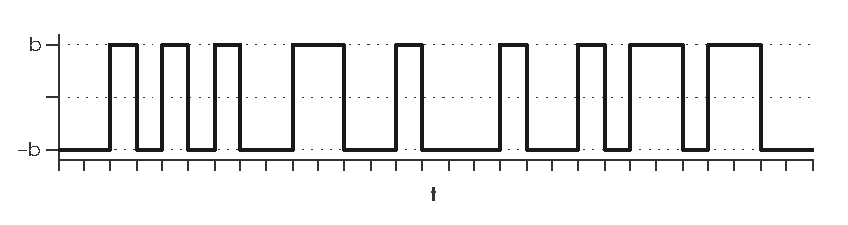
\includegraphics{../fig/general_prbs.eps}
	\caption{A general Pseudo-Random Binary Sequence (PRBS).}
	\label{fig:general_prbs}
\end{figure}

We generated the PRBS signals used for identification by using MATLAB's System Identification Toolbox. Signals were generated for pitch, roll, and yaw rate. Additional input conditioning was performed to appropriately scale the magnitude of the input signal. Scaling factors were experimentally determined to sufficiently excite the vehicle without rendering it uncontrollable.
\begin{figure}[htb!]
	\centering
	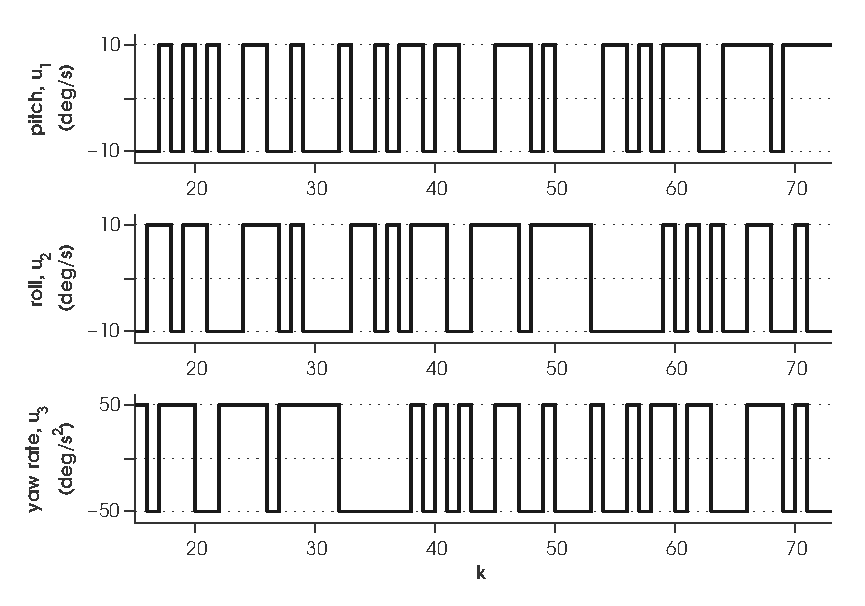
\includegraphics{../fig/test_prbs.eps}
	\caption[A sample PRBS signal used for identification showing scaled inputs for vehicle pitch, roll, and yaw rate.]{A sample PRBS signal used for identification showing scaled inputs for vehicle pitch $= \pm 10^\circ$, roll $= \pm 10^\circ$, and yaw rate $= \pm 50^\circ/\mbox{sec}$.}
\end{figure}

Because the Python API requires system input sequences to be formatted as \{pitch, roll, yaw rate, thrust\}, we also experimentally determined a thrust input which results in vehicle hover. The general flight test sequence is: vehicle power on and sensor calibration, take off and hover, free flight under PRBS input, test conclusion.

FIGURE


Talk about how PRBS goes into controller which in turn generates motor commands
\subsection{Data Collection}





\section{Data Analysis}
INCLUDE OVERVIEW OF IEM ALGORITHM IN BOX (MATH-BASED) IN THIS SECTION

\subsection{Data Preprocessing}

\subsection{Model Identification}

\section{Verification}